%% March 2018
%%%%%%%%%%%%%%%%%%%%%%%%%%%%%%%%%%%%%%%%%%%%%%%%%%%%%%%%%%%%%%%%%%%%%%%%%%%%
% AGUJournalTemplate.tex: this template file is for articles formatted with LaTeX
%
% This file includes commands and instructions
% given in the order necessary to produce a final output that will
% satisfy AGU requirements, including customized APA reference formatting.
%
% You may copy this file and give it your
% article name, and enter your text.
%
%
% Step 1: Set the \documentclass
%
% There are two options for article format:
%
% PLEASE USE THE DRAFT OPTION TO SUBMIT YOUR PAPERS.
% The draft option produces double spaced output.
%

%% To submit your paper:
\documentclass[draft]{agujournal2018}
\usepackage{apacite}
\usepackage{url} %this package should fix any errors with URLs in refs.
\usepackage{lineno}
\linenumbers
%%%%%%%
% As of 2018 we recommend use of the TrackChanges package to mark revisions.
% The trackchanges package adds five new LaTeX commands:
%
%  \note[editor]{The note}
%  \annote[editor]{Text to annotate}{The note}
%  \add[editor]{Text to add}
%  \remove[editor]{Text to remove}
%  \change[editor]{Text to remove}{Text to add}
%
% complete documentation is here: http://trackchanges.sourceforge.net/
%%%%%%%

\draftfalse

%% Enter journal name below.
%% Choose from this list of Journals:
%
% JGR: Atmospheres
% JGR: Biogeosciences
% JGR: Earth Surface
% JGR: Oceans
% JGR: Planets
% JGR: Solid Earth
% JGR: Space Physics
% Global Biogeochemical Cycles
% Geophysical Research Letters
% Paleoceanography and Paleoclimatology
% Radio Science
% Reviews of Geophysics
% Tectonics
% Space Weather
% Water Resources Research
% Geochemistry, Geophysics, Geosystems
% Journal of Advances in Modeling Earth Systems (JAMES)
% Earth's Future
% Earth and Space Science
% Geohealth
%
% ie, \journalname{Water Resources Research}

\journalname{Water Resources Research}


\begin{document}

%% ------------------------------------------------------------------------ %%
%  Title
%
% (A title should be specific, informative, and brief. Use
% abbreviations only if they are defined in the abstract. Titles that
% start with general keywords then specific terms are optimized in
% searches)
%
%% ------------------------------------------------------------------------ %%

% Example: \title{This is a test title}

\title{Partitioning Thresholds in Hybrid Implicit-Explicit Representations of Naturally Fractured Reservoirs}

%% ------------------------------------------------------------------------ %%
%
%  AUTHORS AND AFFILIATIONS
%
%% ------------------------------------------------------------------------ %%

% Authors are individuals who have significantly contributed to the
% research and preparation of the article. Group authors are allowed, if
% each author in the group is separately identified in an appendix.)

% List authors by first name or initial followed by last name and
% separated by commas. Use \affil{} to number affiliations, and
% \thanks{} for author notes.
% Additional author notes should be indicated with \thanks{} (for
% example, for current addresses).

% Example: \authors{A. B. Author\affil{1}\thanks{Current address, Antartica}, B. C. Author\affil{2,3}, and D. E.
% Author\affil{3,4}\thanks{Also funded by Monsanto.}}

\authors{Daniel Wong\affil{1}, Florian Doster\affil{1}, Sebastian Geiger\affil{1}, Arjan Kamp\affil{2}}


% \affiliation{1}{First Affiliation}
% \affiliation{2}{Second Affiliation}
% \affiliation{3}{Third Affiliation}
% \affiliation{4}{Fourth Affiliation}

\affiliation{1}{Institute of Petroleum Engineering, Heriot-Watt University}
\affiliation{2}{Total S.A.}
%(repeat as many times as is necessary)

%% Corresponding Author:
% Corresponding author mailing address and e-mail address:

% (include name and email addresses of the corresponding author.  More
% than one corresponding author is allowed in this LaTeX file and for
% publication; but only one corresponding author is allowed in our
% editorial system.)

% Example: \correspondingauthor{First and Last Name}{email@address.edu}

\correspondingauthor{Daniel Wong}{dlw1@hw.ac.uk}

%% Keypoints, final entry on title page.

%  List up to three key points (at least one is required)
%  Key Points summarize the main points and conclusions of the article
%  Each must be 100 characters or less with no special characters or punctuation

% Example:
% \begin{keypoints}
% \item	List up to three key points (at least one is required)
% \item	Key Points summarize the main points and conclusions of the article
% \item	Each must be 100 characters or less with no special characters or punctuation
% \end{keypoints}

\begin{keypoints}
\item Small fractures up to a threshold size can be lumped with the rock matrix and upscaled into an equivalent porous medium.
\item We determine the threshold size from the relationship between upscaled permeability and the size range of small fractures.
\item Where applicable, the upscaled permeabilities are efficiently established using the Effective Medium Theory compared to numerical upscaling.
\end{keypoints}

%% ------------------------------------------------------------------------ %%
%
%  ABSTRACT
%
% A good abstract will begin with a short description of the problem
% being addressed, briefly describe the new data or analyses, then
% briefly states the main conclusion(s) and how they are supported and
% uncertainties.
%% ------------------------------------------------------------------------ %%

%% \begin{abstract} starts the second page

\begin{abstract}
Fractures can have variable effects on fluid flow in a porous rock. Moderately conductive fractures may enhance the rock’s overall effective permeability while highly conductive fractures may completely dominate fluid transport. Fluid flow modelling is important to quantify the impact of fractures on the performance of a reservoir.  However, simulating fluid flow is computationally intensive due to the heterogeneities introduced by the fracture network. In this work, complex fracture patterns are simplified using hybrid implicit-explicit representations to yield a computationally tractable model. Hybrid modelling requires the selection of a partitioning size to group fractures by size. Small fractures are upscaled with the rock matrix; large fractures are explicitly represented. Our study shows that, given a naturally fractured reservoir, an upper limit exists for the partitioning size and that this threshold partitioning size can be determined without trial and error. Using artificial and realistic fracture patterns, we created hybrid models using different partitioning sizes and subjected them to pressure drawdowns. Simulated production rates were compared against reference results obtained from simulations on the original fracture patterns. Beyond a threshold partitioning size unique to each fracture pattern, hybrid model results deviate significantly from reference solutions. The threshold is identified from the relationship between upscaled permeabilities and partitioning sizes, and corresponds to the point where the effective permeability of small fractures begin to increase rapidly. The permeability-size relationship is obtained using numerical flow-based upscaling. For uniformly distributed fractures with no abutment relationships, the Effective Medium Theory is shown to generate accurate permeability-size relationships. (250 words)

\end{abstract}

\textbf{Plain Language Summary:} Naturally fractured reservoirs are exploited in several industries as they (1) may contain oil and gas, (2) can also be used to extract heat from underground, (3) form pathways for groundwater to flow, (4) can be used to store CO2 and mitigate climate change. As such, it is important to predict how fluids will move through such reservoirs. This is difficult because fractured reservoirs contain fractures that differ greatly in size. One approach that alleviates this problem is to represent the rock and smaller fractures by an equivalent rock that has a comparable flow behaviour. Our study finds that this approach works, but there is a limit to what can be considered small. When this simplification is applied to fractures that are larger than the limit, the resulting equivalent representation fails to capture the correct flow behaviour. We show that the limit can be pre-determined by studying how the equivalent rock properties change with the size range of small fractures. We also show that this procedure can be carried out efficiently using a technique called the Effective Medium Theory. The findings in this study will allow industry practitioners to systematically simplify their fractured reservoir flow modelling problems.



%% ------------------------------------------------------------------------ %%
%
%  TEXT
%
%% ------------------------------------------------------------------------ %%

%%% Suggested section heads:
% \section{Introduction}
%
% The main text should start with an introduction. Except for short
% manuscripts (such as comments and replies), the text should be divided
% into sections, each with its own heading.

% Headings should be sentence fragments and do not begin with a
% lowercase letter or number. Examples of good headings are:

% \section{Materials and Methods}
% Here is text on Materials and Methods.
%
% \subsection{A descriptive heading about methods}
% More about Methods.
%
% \section{Data} (Or section title might be a descriptive heading about data)
%
% \section{Results} (Or section title might be a descriptive heading about the
% results)
%
% \section{Conclusions}


\section{Introduction}
Naturally fractured reservoirs are abundant in nature and of great interest in areas including but not limited to hydrocarbon extraction, geothermal energy production and underground water resources exploitation \citep{Berkowitz2002}. More recently, there has also been 
interest in fractured reservoirs as potential sites for carbon sequestration \citep{March2018}. In all these applications, the central process at play is fluid flow in fractured porous media, and accurately modelling this process is crucial for engineering success.

However, the highly heterogeneous nature of fractured reservoirs makes flow modelling difficult. Instead of representing all fractures in a simulation model, a popular approach, known as the continuum method, is to represent the fracture network as equivalent porous media. The conversion from discrete fractures to a continuum representation involves a process known as upscaling. Depending on the type of fracture system, various continuum models can be constructed via different approaches \citep{Berkowitz2002,Berre2018a}.

For fracture networks in an impermeable background matrix, flow only occurs in fractures. In particular, flow is predominantly facilitated by the hydraulic backbone of a fracture network. Such systems are usually represented as a single continuum via one of two upscaling approaches: geometry or flow based. In geometry based upscaling, a grid is superposed on the fracture network, and the fracture network conductivity is mapped onto the grid based on intersections between fractures and grid cell boundaries \citep{Botros2008, Roubinet2010, Svensson2001}. Flow based upscaling, on the other hand, employs local steady-state solutions to the Laplace problem to back-calculate effective permeabilities using Darcy's law. This can be done numerically through simulations on the grid cell scale \citep{Durlofsky1991, Jackson2000}. Alternatively, \citet{Oda1985} provides an analytical approach to flow based upscaling of well connected networks, which does not require any simulations.

Instead of an impermeable matrix, the focus of this paper is on fractured porous media, which are complicated by the presence of significant matrix permeability, resulting in distinctive time scales for flow in fractures and the matrix. Moreover, unconnected fractures are now able to communicate through the matrix, making a hydraulic backbone difficult to identify \citep{Matthai2004a}. For well connected fracture networks, dual porosity and dual permeability models are often used; these models represent the fractures and matrix as separate continua that interact with each other through transfer functions. Dual porosity models assume no communication between matrix blocks, while dual permeability models allow flow between matrix blocks \citep{Lemonnier2010, Warren1963}. Upscaling of the fractures into a secondary continuum can be performed using the same methods employed for flow in fractured impermeable media. 

If a fracture network is poorly connected, a single continuum representation, in which fractures are upscaled alongside the matrix, can be used \citep{Berre2018a}. In such cases, only flow based upscaling can be employed since the geometrical approach is unable to account for matrix flow. The upscaling procedure can be performed numerically using the method proposed by \citet{Durlofsky1991} for general heterogeneous permeability fields. Alternatively, analytical flow based upscaling can be performed using Oda's method or the Effective Medium Theory; the latter was recently adapted for fractured porous media and has been shown to outperform Oda's method. This is because the Effective Medium Theory directly addresses the effects of fracture sizes on upscaled permeabilities while Oda's method assumes fractures have infinite length, which automatically implies well-connectedness \citep{Oda1985, Saevik2013, Saevik2014}. More recently, a variant of flow based upscaling known as aggregation based upscaling was introduced by \citet{Hui2017}. In this approach, a steady state single phase flow simulation is first performed for a finely gridded model. The fine cells are then aggregated into coarse cells. Transmissibilities between coarse cells are derived using fluxes obtained from the steady state single phase flow simulation. For this work, numerical upscaling is performed using the method proposed by \citet{Durlofsky1991} due to its ease of implementation and wider usage. 

In practice, continuum methods are increasingly being used in conjunction with Discrete Fracture and Matrix (DFM) methods, which explicitly represent fractures in permeable rocks. Such methods are collectively termed hybrid methods and can involve various continuum-DFM method combinations. One such model is the single porosity hybrid model; this model represents small scale fractures and the matrix using a single continuum - sometimes called a pseudo-matrix - and explicitly represents large fractures \citep{Lee2001, Li2008, Rogers2007}. The single porosity hybrid model can be viewed as a simplified DFM model with reduced complexity. Within the framework of hybrid models, single porosity hybrid models are the simplest possible hybrid models. More complex models that couple DFM and multi-continuum approaches have also been developed. For example, \citet{Jiang2015} proposed a dual permeability hybrid model which combines DFM and the dual permeability model. While complex hybrid models have been shown to produce accurate results, they are computationally more expensive. Hence, simpler hybrid models are preferred if they are applicable. The main motivation for the shift towards hybrid models is that fractured reservoirs tend to exhibit multiple length scales; upscaling on a grid cell basis will under-represent the highly conductive nature of fractures larger than the cell size. Ideally, full fracture network representation through DFM methods would circumvent errors arising from upscaling. However, limitations on computational resources necessitates the use of continuum methods in conjunction with DFM methods.

While promising, the introduction of hybrid methods opens up further questions regarding how they should be constructed. In particular, which fractures should be upscaled and which ones should be explicitly modelled? How many continua should the upscaled fractures be represented with? Which continuum should each fracture belong to? In our work, we apply a bottom up approach by investigating the applicability of single porosity hybrid models for flow modelling in fractured porous media. In all single porosity hybrid models, the fracture network has to be partitioned into two sets: one set with fracture sizes less than the partitioning size, and another with larger fractures. Using either numerical or analytical flow based upscaling, equivalent porous media with effective permeabilities are derived to implicitly account for flow in small fractures and the rock matrix. Meanwhile, the large fractures are explicitly represented. It should be noted that, here, we are not proposing a new single porosity hybrid method. On the contrary, the outlined process of constructing a single porosity hybrid model is similar no matter what DFM or upscaling approach is used. Instead of comparing different types of single porosity hybrid models, the focus of our work is on determining when the single porosity hybrid modelling approach can be applied. Constructing a hybrid model using a small partitioning size preserves as many details as possible, at the expense of computational efficiency. On the other hand, large partitioning sizes yield significant model simplifications, but at the cost of model accuracy.

In this paper, we explore the relationships between effective permeabilities and partitioning sizes using various fracture networks. We observe from these relationships that there exists threshold partitioning sizes beyond which effective permeabilities increase rapidly. We propose an algorithm for determining the threshold partitioning size corresponding to each fractured reservoir. We further hypothesize that for a fractured reservoir, single porosity hybrid models should only be constructed using partitioning sizes below the corresponding threshold. To verify this, we compare the performances of hybrid models created using various partitioning sizes against full model solutions. The results ascertain that hybrid models can indeed be used to simplify complex fractured reservoir simulations if partitioning sizes are below observed thresholds. Additionally, we also show that the permeability-size relationship can be produced efficiently using the Effective Medium Theory. This approach enables fast calculations of threshold partitioning sizes. If additional geological features such as fracture abutment relationships or non-uniform spatial distributions need to be considered, the slower numerical flow based upscaling approach, which is less restrictive in terms of fracture network properties, can also be used.

\section{Methods}

In this section, we elaborate on the methods used to generate Discrete Fracture Networks (DFN) for the purpose of our studies. The DFNs are converted into simulation models for flow modelling. The first set of flow simulations performed are incompressible single phase flow. These simulations allow us to conduct numerical upscaling of the DFNs. Additionally, for some DFNs, the upscaling results are reproduced using the Effective Medium Theory. In this section, we also outline the procedure for determining threshold partitioning sizes for each DFN based on the outputs from the upscaling procedure. Finally, we create hybrid simulation models for each DFN. The full and hybrid models are subjected to pressure drawdowns to simulate production responses, which can then be compared against each other. The comparison of the production responses allow us to evaluate how well a hybrid model represents a fully resolved model.

\subsection{Data}
The Discrete Fracture Networks (DFN) used in this study are either (1) generated in 3D using the procedures laid out in \citet{Priest1993}, or (2) based on realistic 2D fracture networks (Figure \ref{fig:DD}) \citep{Bisdom2015, Bisdom2017}.

For each 3D DFN, three orthogonal sets of circular fractures are generated stochastically in a 100m x 100m x 100m cubic domain by drawing from a power law distribution for size and uncorrelated uniform distribution in space. The base parameters used are the fracture density ($P_{32}=0.15$m\textsuperscript{2}/m\textsuperscript{3} per fracture set), the power law exponent of fracture sizes ($n_s=1.5$), and the fracture size range ($s_{min}=5$m and $s_{max}=20$m in radii) \citep{Bonnet2001, Dershowitz1992, Ebigbo2016}. Fractures are prevented from being unrealistically close to each other using 1\% of fracture size as a minimum distance. Fracture apertures vary with size, following an aperture-size ratio of $3.5\times 10^{-5}$, which was chosen to ensure that fracture apertures were close to 1mm, as observed by \citet{Bisdom2015}. Aperture is used to calculate fracture intrinsic permeabilities using the cubic law \citep{Witherspoon1980}. Rock permeability used is $K_m=10$mD. Four different cases are considered here: (A) Base case using the presented parameters, (B) $2\times P_{32}$, (C) $2\times n_s$ and (D) $2\times s_{max}$. Examples of these DFNs are shown in Figure \ref{fig:DD}, with each example containing respectively 1785, 3610, 2607 and 879 fractures. Additionally, nine other cases were also studied; the parameters used are documented in Text S1 and Table S1.

The 2D DFNs are created from a publicly available dataset containing trace maps of fractures observed on outcrops of the Jandaira Carbonate Formation in Brazil. The trace maps used in this study are the Apodi 2 and 4 maps, named after the municipality where the outcrop is located. Both fracture networks are multiscale in nature and exhibit fracture sizes (lengths) ranging across two orders of magnitude \citep{Bisdom2015}. The model sizes of the two DFNs are 220m x 220m and 100m x 100m for Apodi 2 and 4 respectively. As no reliable aperture information were obtained for these fracture networks, we account for the variability in fracture apertures by assuming an aperture-size ratio of $3.5\times 10^{-5}$ to keep the largest aperture (corresponding to a fracture length of 218m) below 10mm. The smallest aperture (corresponding to a fracture length of 1.1m) is 38.7 microns. Fracture permeabilities are evaluated using the cubic law. Rock permeability used is $K_m=1$mD. The fracture networks are shown in Figures \ref{fig:DD}, with Apodi 2 containing 298 fractures and Apodi 4 containing 546 fractures.

\subsection{Fully Resolved Models}
The simulations in this paper are performed using the Embedded Discrete Fracture Model (EDFM), which is available through the MATLAB Reservoir Simulation Toolbox (MRST) \citep{Lie2012, Shah2016}. This implementation of EDFM allows matrix grids to be independently constructed, while the fractures grids are constructed based on intersections between fractures and matrix cells. Non-neighbouring connections (NNC) are used to facilitate fracture-matrix and fracture-fracture flow \citep{Lee2001, Li2008, Moinfar2014}. Fully resolved models are created from the 2D and 3D DFNs using the EDFM module in MRST. These models will be used to generate reference simulations to compare hybrid model simulations against. The number of grid cells and NNCs for each fully resolved model is shown in Table \ref{tab:gridstats}.

\begin{table}[htb]
	\centering
	\begin{tabular}{| c | c | c | c |}
		\hline
		Name & Matrix cells & Fracture cells & NNCs\\
		\hline
		A & 15625 & 42101 & 67033\\
		B & 15625 & 84015 & 182589\\
		C & 15625 & 45919 & 72726\\
		D & 15625 & 36503 & 58568\\
		Apodi 2 & 56644 & 8804 & 10107\\
		Apodi 4 & 68906 & 16806 & 20651\\
		\hline
	\end{tabular}
\caption{Number of grid cells and NNCs for the fully resolved simulation models of the 2D and 3D DFNs.}
\label{tab:gridstats}
\end{table}

\subsection{Fracture Subset Upscaling}
To create a hybrid model, we first need to upscale all fractures smaller than a selected partitioning size, $s_p$ - we call this Fracture Subset Upscaling (FSU) (Figure \ref{fig:FSU_Scheme}). FSU using EDFM is done by solving the Laplace equation for a square domain containing only fractures with sizes in $[s_{min},s_p]$, subject to a pressure differential on two opposing boundaries, and no-flow condition on the remaining boundaries. From a simulation standpoint, fractures that are larger than $s_p$ can simply be deactivated to exclude them from the flow domain. The simulation yields a flow field that can be used to calculate an effective permeability, $K_{e}$, using Darcy's law. The calculated $K_{e}$ is a function of $s_p$. The results are summarized in FSU curves (Figures \ref{fig:FSU} and S1) that plot $K_{e}/K_m$ against $s_p$, where $K_m$ is rock matrix permeability.

\begin{figure}[h]
	\centering
	
	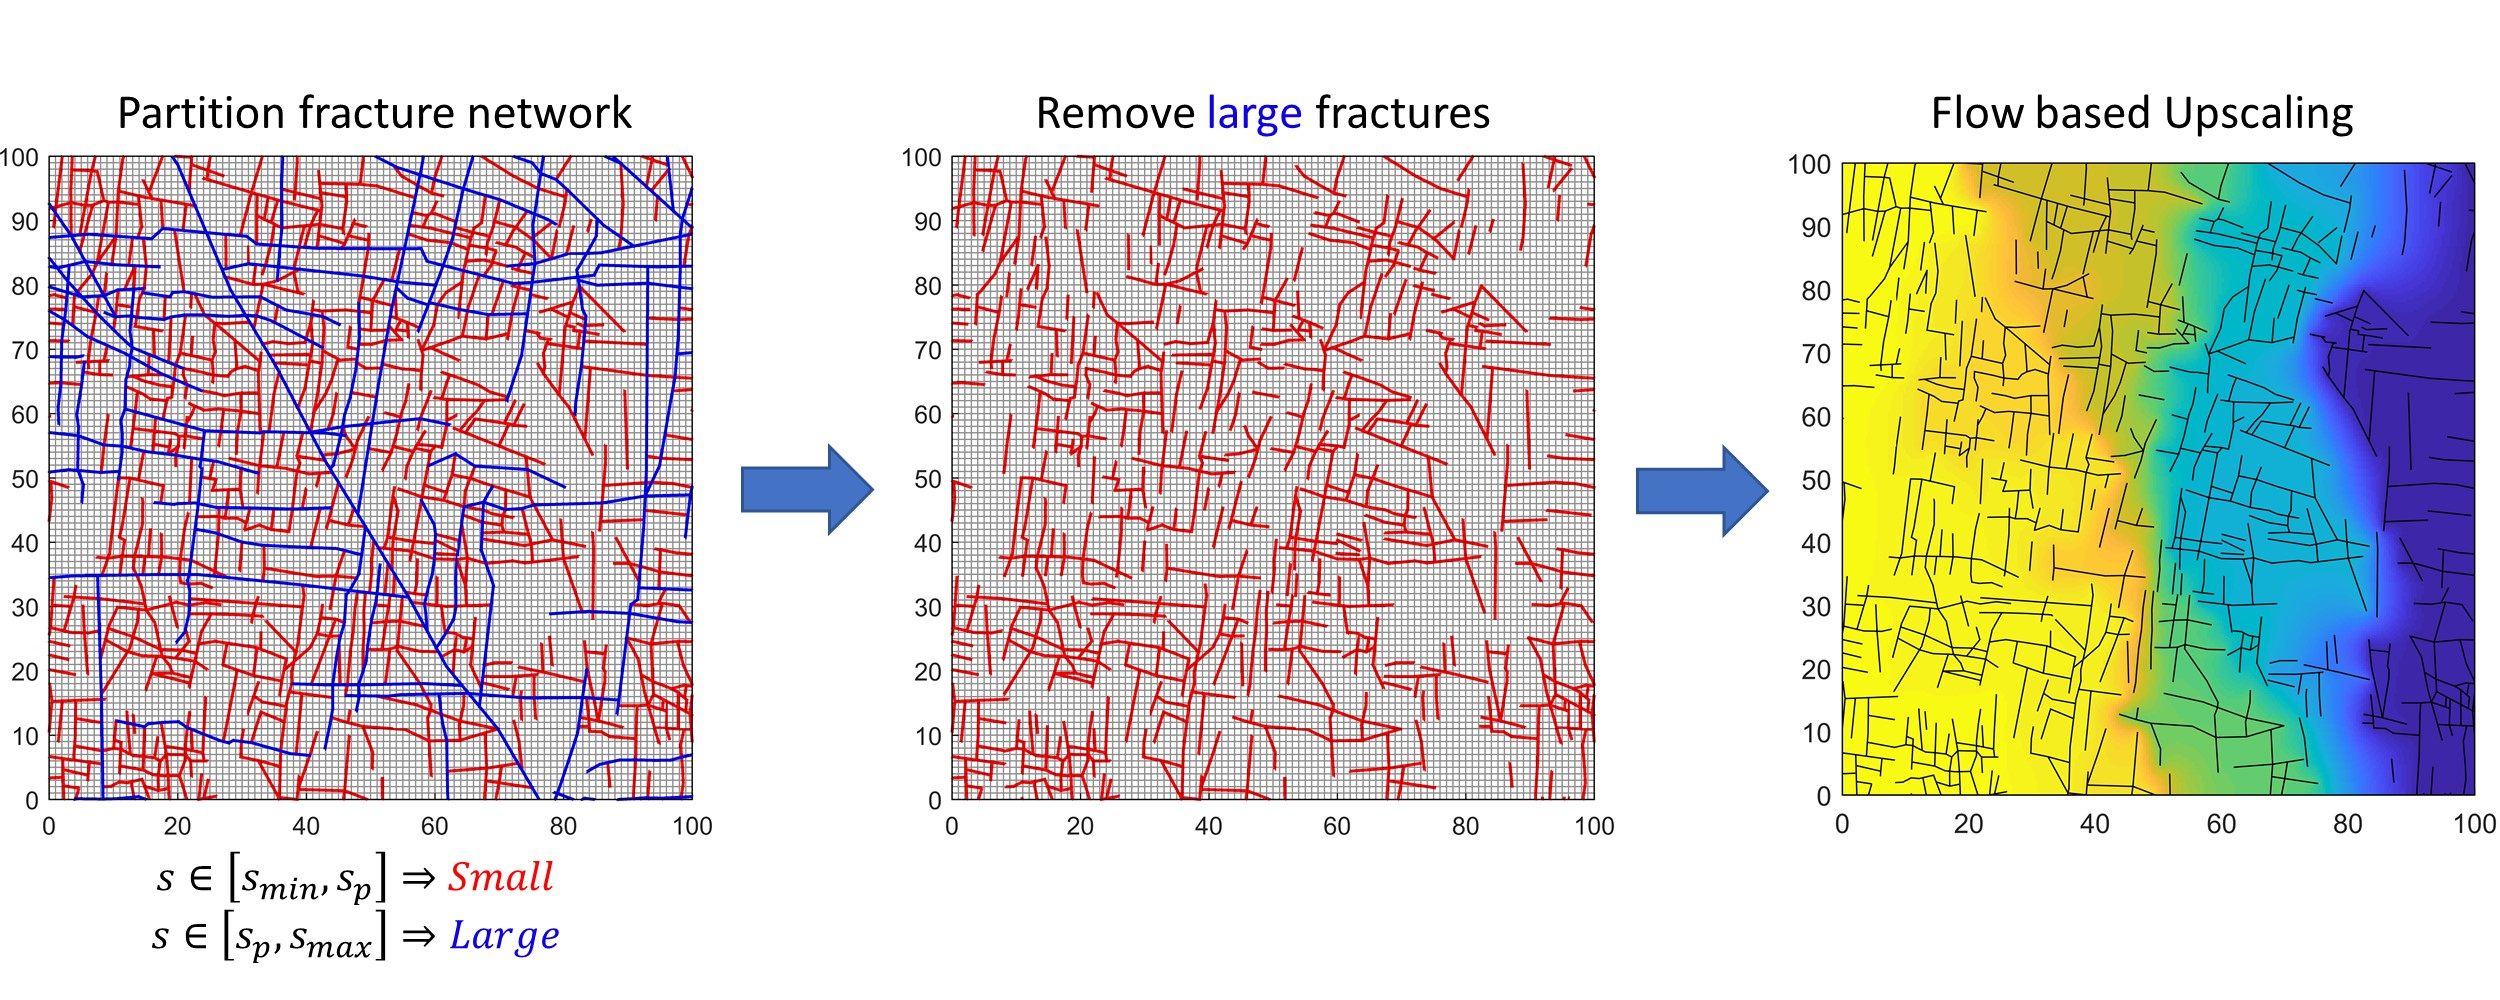
\includegraphics[width=\textwidth]{FSU_Scheme.jpg}
	
	\caption{Illustration of the Fracture Subset Upscaling procedure. Given a fracture network and a user defined partitioning size, sp, fractures larger then sp are removed. Remaining small fractures are upscaled using either a numerical or analytical flow based approach. The entire process is repeated for different partitioning sizes to capture the relationship between effective permeability and partitioning size.}
	\label{fig:FSU_Scheme}
\end{figure}

For the 3D DFNs, FSU was also performed using the Effective Medium Theory \citep{Saevik2013}. Two main methods of the theory are considered, namely the asymmetric self-consistent method

\begin{equation}
K_e=K_m+ \frac{4}{3} \pi \sum_{1}^{N} \varepsilon_i(\lambda_i B_i (K_e)+I)^{-1}B_i(K_e),
\label{eqn:AEMT}
\end{equation}

and the symmetric self-consistent method

\begin{equation}
K_e=K_m+ \frac{4}{3} \pi \sum_{1}^{N} \frac{\varepsilon_i}{v_m}(\lambda_i B_i (K_e)+I)^{-1}B_i(K_e)R_m(K_m)^{-1},
\label{eqn:SEMT}
\end{equation}

where $\varepsilon$, $\lambda$, $v$ refer respectively to dimensionless fracture density, dimensionless fracture permeability and volume fraction. The indices $i\in[1,N]$ refer to different fracture sets. $B$ and $R$ are tensor functions whose parameters are the shape and orientation of the corresponding fracture set. We refer the reader to \citet{Saevik2013} for the derivation of equations \ref{eqn:AEMT} and \ref{eqn:SEMT} as well as the expressions for $\varepsilon$, $\lambda$, $B$ and $R$.

The symmetric self-consistent method differs from its asymmetric counterpart in that it mathematically represents the matrix as an equivalent fracture set in its derivation \citep{Barthelemy2009, Saevik2013}. This has been shown to improve results at low fracture densities. However, the asymmetric self-consistent method better predicts percolation thresholds \citep{Saevik2013, Saevik2014}.

While equations \ref{eqn:AEMT} and \ref{eqn:SEMT} were developed for monodisperse fracture families which contain only fractures with no variation in orientation, they can be extended for polydisperse fracture families. \citet{Ebigbo2016} showed results of the application of the Effective Medium Theory on polydisperse fracture families. However, no methodology was provided as to how equations \ref{eqn:AEMT} and \ref{eqn:SEMT} were adapted. Here, we demonstrate how we apply the Effective Medium Theory to polydisperse fracture families through the asymmetric self-consistent method. The same solution strategy can be used for the symmetric self-consistent method. 

First, we consider a single polydisperse fracture family that has continuously distributed fracture sizes. We can then define a fracture density function $\varepsilon(s)$ such that $\varepsilon(s)\ ds$ is the $P_{31}$ density of fractures with sizes within $[s,s+ds]$. In this work, the fracture density function used is $\varepsilon (s)=\alpha s^{-a}$, which follows a power law distribution \citep{Bonnet2001}. In line with the assumed linear aperture-size relationship and the cubic law, we also let the intrinsic fracture permeability depend on fracture size, such that $\lambda=\lambda (s)$. Since the shapes and orientations of all fractures are fixed, $B$ remains constant.

For this fracture family, we can rewrite equation \ref{eqn:AEMT} in continuous form as
\begin{equation}
K_e =  K_m + \frac{4}{3} \pi \int_{s_{min}}^{s_{max}} \varepsilon (s) \left(\lambda (s) B + I\right)^{-1}B\ ds.
\end{equation}
If there are $N_f$ polydisperse fracture families, we can sum up their contributions to arrive at
\begin{equation}
\label{eqn:polydisperse_aEMT}
K_e =  K_m + \frac{4}{3} \pi \sum_{i=1}^{N_f} \left[ \int_{s_{i,min}}^{s_{i,max}} \varepsilon_i (s) \left(\lambda_i (s) B_i + I\right)^{-1}B_i\ ds \right],
\end{equation}
where each fracture family $i$ has fracture sizes ranging from $s_{i,min}$ to $s_{i,max}$, a fracture density function $\varepsilon_i (s)$ and a permeability-size relationship $\lambda_i (s)$.

To perform FSU with equation \ref{eqn:polydisperse_aEMT}, we only account for contributions from fractures smaller than a partitioning size $s_p$. So we substitute $s_{i,max}$ with $s_p$ to obtain
\begin{equation}
\label{eqn:FSU_aEMT}
K_e =  K_m + \frac{4}{3} \pi \sum_{i=1}^{N_f} \left[ \int_{s_{i,min}}^{s_p} \varepsilon_i (s) \left(\lambda_i (s) B_i + I\right)^{-1}B_i\ ds \right],
\end{equation}
which can be used to solve for effective permeabilities. 

However, equation \ref{eqn:FSU_aEMT} is an implicit equation in $K_e$ and it is not obvious how the integral terms can be analytically solved. Hence, we approximate each polydisperse fracture family as a set of $N_{sf}$ monodisperse fracture sub-families. For a particular polydisperse fracture family $i$, we perform the following:

\begin{enumerate}
	\item Calculate sub-family size range $\delta s_i = \left(s_p - s_{i,min}\right)/N_{sf}$.
	\item For each sub-family $j=1,2,....,N_{sf}$
	\begin{enumerate}
		\item Determine the representative fracture size $s_{i,j} = s_{i,min} + \left(j-0.5\right) \delta s_i$.
		\item Calculate the sub-family dimensionless intrinsic fracture permeability $\lambda_{i,j}=\lambda_i(s_{i,j})$.
		\item Calculate the sub-family fracture density $$\varepsilon_{i,j}=\int_{ s_{i,min} + \left(j-1\right) \delta s_i}^{ s_{i,min} + j\delta s_i} \varepsilon_i (s)\ ds.$$
	\end{enumerate}	
\end{enumerate}

This procedure results in a total of $N_f \times N_{sf}$ fracture sub-families. The first $N_{sf}$ sub-families are generated from the first fracture family. The next $N_{sf}$ sub-families are generated from the second fracture family, and so on. The construction of the monodisperse sub-families allows us to make the following approximation
\begin{equation}
\label{eqn:powerlaw_approx}
\int_{s_{i,min}}^{s_p} \varepsilon_i (s) \left(\lambda_i (s) B_i + I\right)^{-1}B_i\ ds 
\approx \sum_{j=1}^{N_{sf}} \varepsilon_{i,j} \left(\lambda_{i,j} B_i + I\right)^{-1}B_i,
\end{equation}
for all $i \in \{1,2,...,N_f\}$. Substituting \ref{eqn:powerlaw_approx} into \ref{eqn:FSU_aEMT}, we arrive at
\begin{equation}
\label{eqn:FSU_aEMT_approx}
K_e =  K_m + \frac{4}{3} \pi \sum_{i=1}^{N_f} \sum_{j=1}^{N_{sf}} \varepsilon_{i,j} \left(\lambda_{i,j} B_i + I\right)^{-1}B_i.
\end{equation}

Applying the same procedure to the symmetric self-consistent method, we obtain
\begin{equation}
\label{eqn:FSU_sEMT_approx}
K_e =  K_m + \frac{4}{3} \pi \sum_{i=1}^{N_f} \sum_{j=1}^{N_{sf}} \frac{\varepsilon_{i,j}}{v_m} \left(\lambda_{i,j} B_i + I\right)^{-1}B_i R_m^{-1}.
\end{equation}

Note that equations \ref{eqn:FSU_aEMT_approx} and \ref{eqn:FSU_sEMT_approx} have the same form as the standard Effective Medium Theory equations \ref{eqn:AEMT} and \ref{eqn:SEMT}. Hence, the monodisperse fracture sub-families can simply be re-indexed and used with the standard equations to calculate effective permeabilities.

We performed FSU for the 3D DFNs using equations \ref{eqn:FSU_aEMT_approx} and \ref{eqn:FSU_sEMT_approx} with $N_{sf}=1000$ to ensure the method converges. The results are shown in Figures \ref{fig:FSU} and S1. It is worth noting that FSU using the Effective Medium Theory does not involve DFNs themselves. Instead, the inputs for the Effective Medium Theory are the parameters used to generate the DFNs. Since the DFNs that we have used in this study are only one stochastic realization of each parameter set, we further generated nine stochastic realizations for each case studied. Numerical FSU was performed for these stochastic realizations and the results are included in Figures \ref{fig:FSU} and S1. The results from the additional stochastic realizations allow us to verify that the FSU curves generated from the Effective Medium Theory are applicable to all the realizations. The additional stochastic realizations are not used for any subsequent simulations in this work.

\subsection{Calculation of Threshold Partitioning Sizes}
As will be shown in the results section, FSU allows us to observe threshold partitioning sizes beyond which effective permeabilities begin to increase rapidly. Here, we outline a quantitative algorithm for determining the threshold partitioning sizes. Note that the same algorithm works for both numerical and analytical FSU. Given $\left(s_p,K_{e}/K_m\right)$ pairs calculated from numerical or analytical FSU, we perform the following:
\begin{enumerate}
	\item Calculate $\log(K_{e}/K_m)$ for each $s_p$.
	\item Calculate the numerical first and second derivatives of $\log(K_{e}/K_m)$ with respect to $s_p$ using the central difference scheme. Forward or backward difference schemes are used for the end points.
	\item Calculate the radius of curvature for $\log(K_{e}/K_m)$ with respect to $s_p$ using the first and second derivatives calculated in the preceding step.
	\item Fit a quadratic curve to the first calculated local minimum and its adjacent points.
	\item $s_p$ at the minimum point on the quadratic curve is the threshold partitioning size $s_p^*$.
\end{enumerate}

For each 2D outcrop-based model, thresholds were calculated using the FSU curves for both the x- and y- directions. The final $s_p^*$ is the average of the two. For each 3D DFN, since FSU was performed both numerically and analytically, $s_p^*$ corresponding to each approach is calculated. The calculated $s_p^*$ values are indicated in Figures \ref{fig:FSU} and S1.

\subsection{Hybrid Models}
Given $s_p$, once small fractures are upscaled to obtain $K_e$, a hybrid model containing only fractures ranging from $[s_p,s_{max}]$ can be constructed. The background permeability used in the hybrid model is $K_e$ instead of $K_m$. Using the FSU curves in Figures \ref{fig:FSU} and S1, for each dataset, we created a set of hybrid models corresponding to different $s_p$. These models will be used to evaluate the impact of different partitioning choices on the accuracy of hybrid representations.

The hybrid models, along with the original full DFN model, are subjected to drawdowns in order to compare their performances. The 3D DFN models are tested using fixed pressure boundary conditions while the 2D outcrop-based models are tested using a single well with fixed production rate (Figure \ref{fig:DD} and S3). The different drawdown conditions are used to test the robustness of our findings. In all cases, initial pressure is $100$bars and typical oil properties are used ($\rho_o=700$kg/m\textsuperscript{3}, $\mu_o=5$cP, $c_o=10^{-5}$bars\textsuperscript{-1}). The results of these drawdown tests are shown in Figures \ref{fig:DD}, S2 and S3. 

To compare the performance of hybrid models to the fully resolved models, the mismatch between hybrid and reference model solutions are also calculated at selected points in time (Figure \ref{fig:HP}).  The calculation of the mismatch is as follows
\begin{equation}
e(s_p)=\left|\frac{X(s_p)-X_{ref}}{X_{ref}}\right|,
\end{equation}
where $X$ refers to either flowrate or pressure derivative, depending on the type of drawdown simulated. $X_{ref}$ corresponds to the results generated by the fully resolved models.

Additionally, for each $s_p$, model simplification is measured through the reduction in the number of fractures, the number of fracture grid cells, and the number of NNCs (Figure \ref{fig:HP}). The number of fractures in a hybrid model is expected to be less than the corresponding fully resolved model since fractures smaller than $s_p$ have been upscaled. Consequently, the number of fracture grid cells are reduced. With less fractures, the number of NNCs is also reduced. The reduction of grid cells and NNCs will both ease the computational load on the reservoir simulator's linear solver. The calculations for model simplification are performed using the following equation
\begin{equation}
\Delta Y(s_p) = \frac{Y(s_p)}{Y_{ref}},
\end{equation}
where $Y$ refer to either the number of fractures, the number of fracture grid cells, or the number of NNCs.

\section{Results}
\subsection{Effective Permeability and Partitioning Size}
Numerical FSU results are shown in Figure \ref{fig:FSU} for the four 3D cases and outcrop-based DFNs. Results for the additional 3D cases are shown in Figure S1. These curves establish the relationship between upscaled permeabilities and partitioning sizes. While they are mainly used in our study to facilitate hybrid model construction, we make some noteworthy observations.

% Last sentence above is optional. Remove if limited words.

The FSU curves show that $K_e/K_m$ increases monotonically with $s_p$. This is because as $s_p$ increases, the size range of fractures that are upscaled increases, resulting in a denser set of fractures. This naturally enhances the overall connectivity and conductivity of the fracture network.

It can also be observed that the FSU curves show a percolation behaviour, where $K_e$ suddenly increases rapidly past some threshold $s_p^*$. This implies that with low $s_p$ values, fracture subsets are not well connected, but as $s_p$ increases, not only does the number of fractures in the subset increase, but the connectivity of the fracture subset increases as well. Calculated $s_p^*$ values are shown in Figures \ref{fig:FSU} and S1. We hypothesize that single porosity hybrid modelling is only applicable when $s_p\leq s_p^*$.

The 3D cases are also used to illustrate how the shape of FSU curves depends on fracture network properties. When the fracture density is doubled (Case B), the resulting fracture subset contains more fractures for the same $s_p$. This is reflected in the FSU curve which shows higher overall $K_e$ and an earlier transition to large $K_e$. In Case C, the power law size exponent is doubled. Hence the proportion of small sized fractures is higher, which causes the fracture subset to percolate earlier. In Case D, the range of fracture sizes is larger. Subsequently, $K_e$ begins to increase rapidly from a larger $s_p$.

\begin{figure}[h]
 \centering

 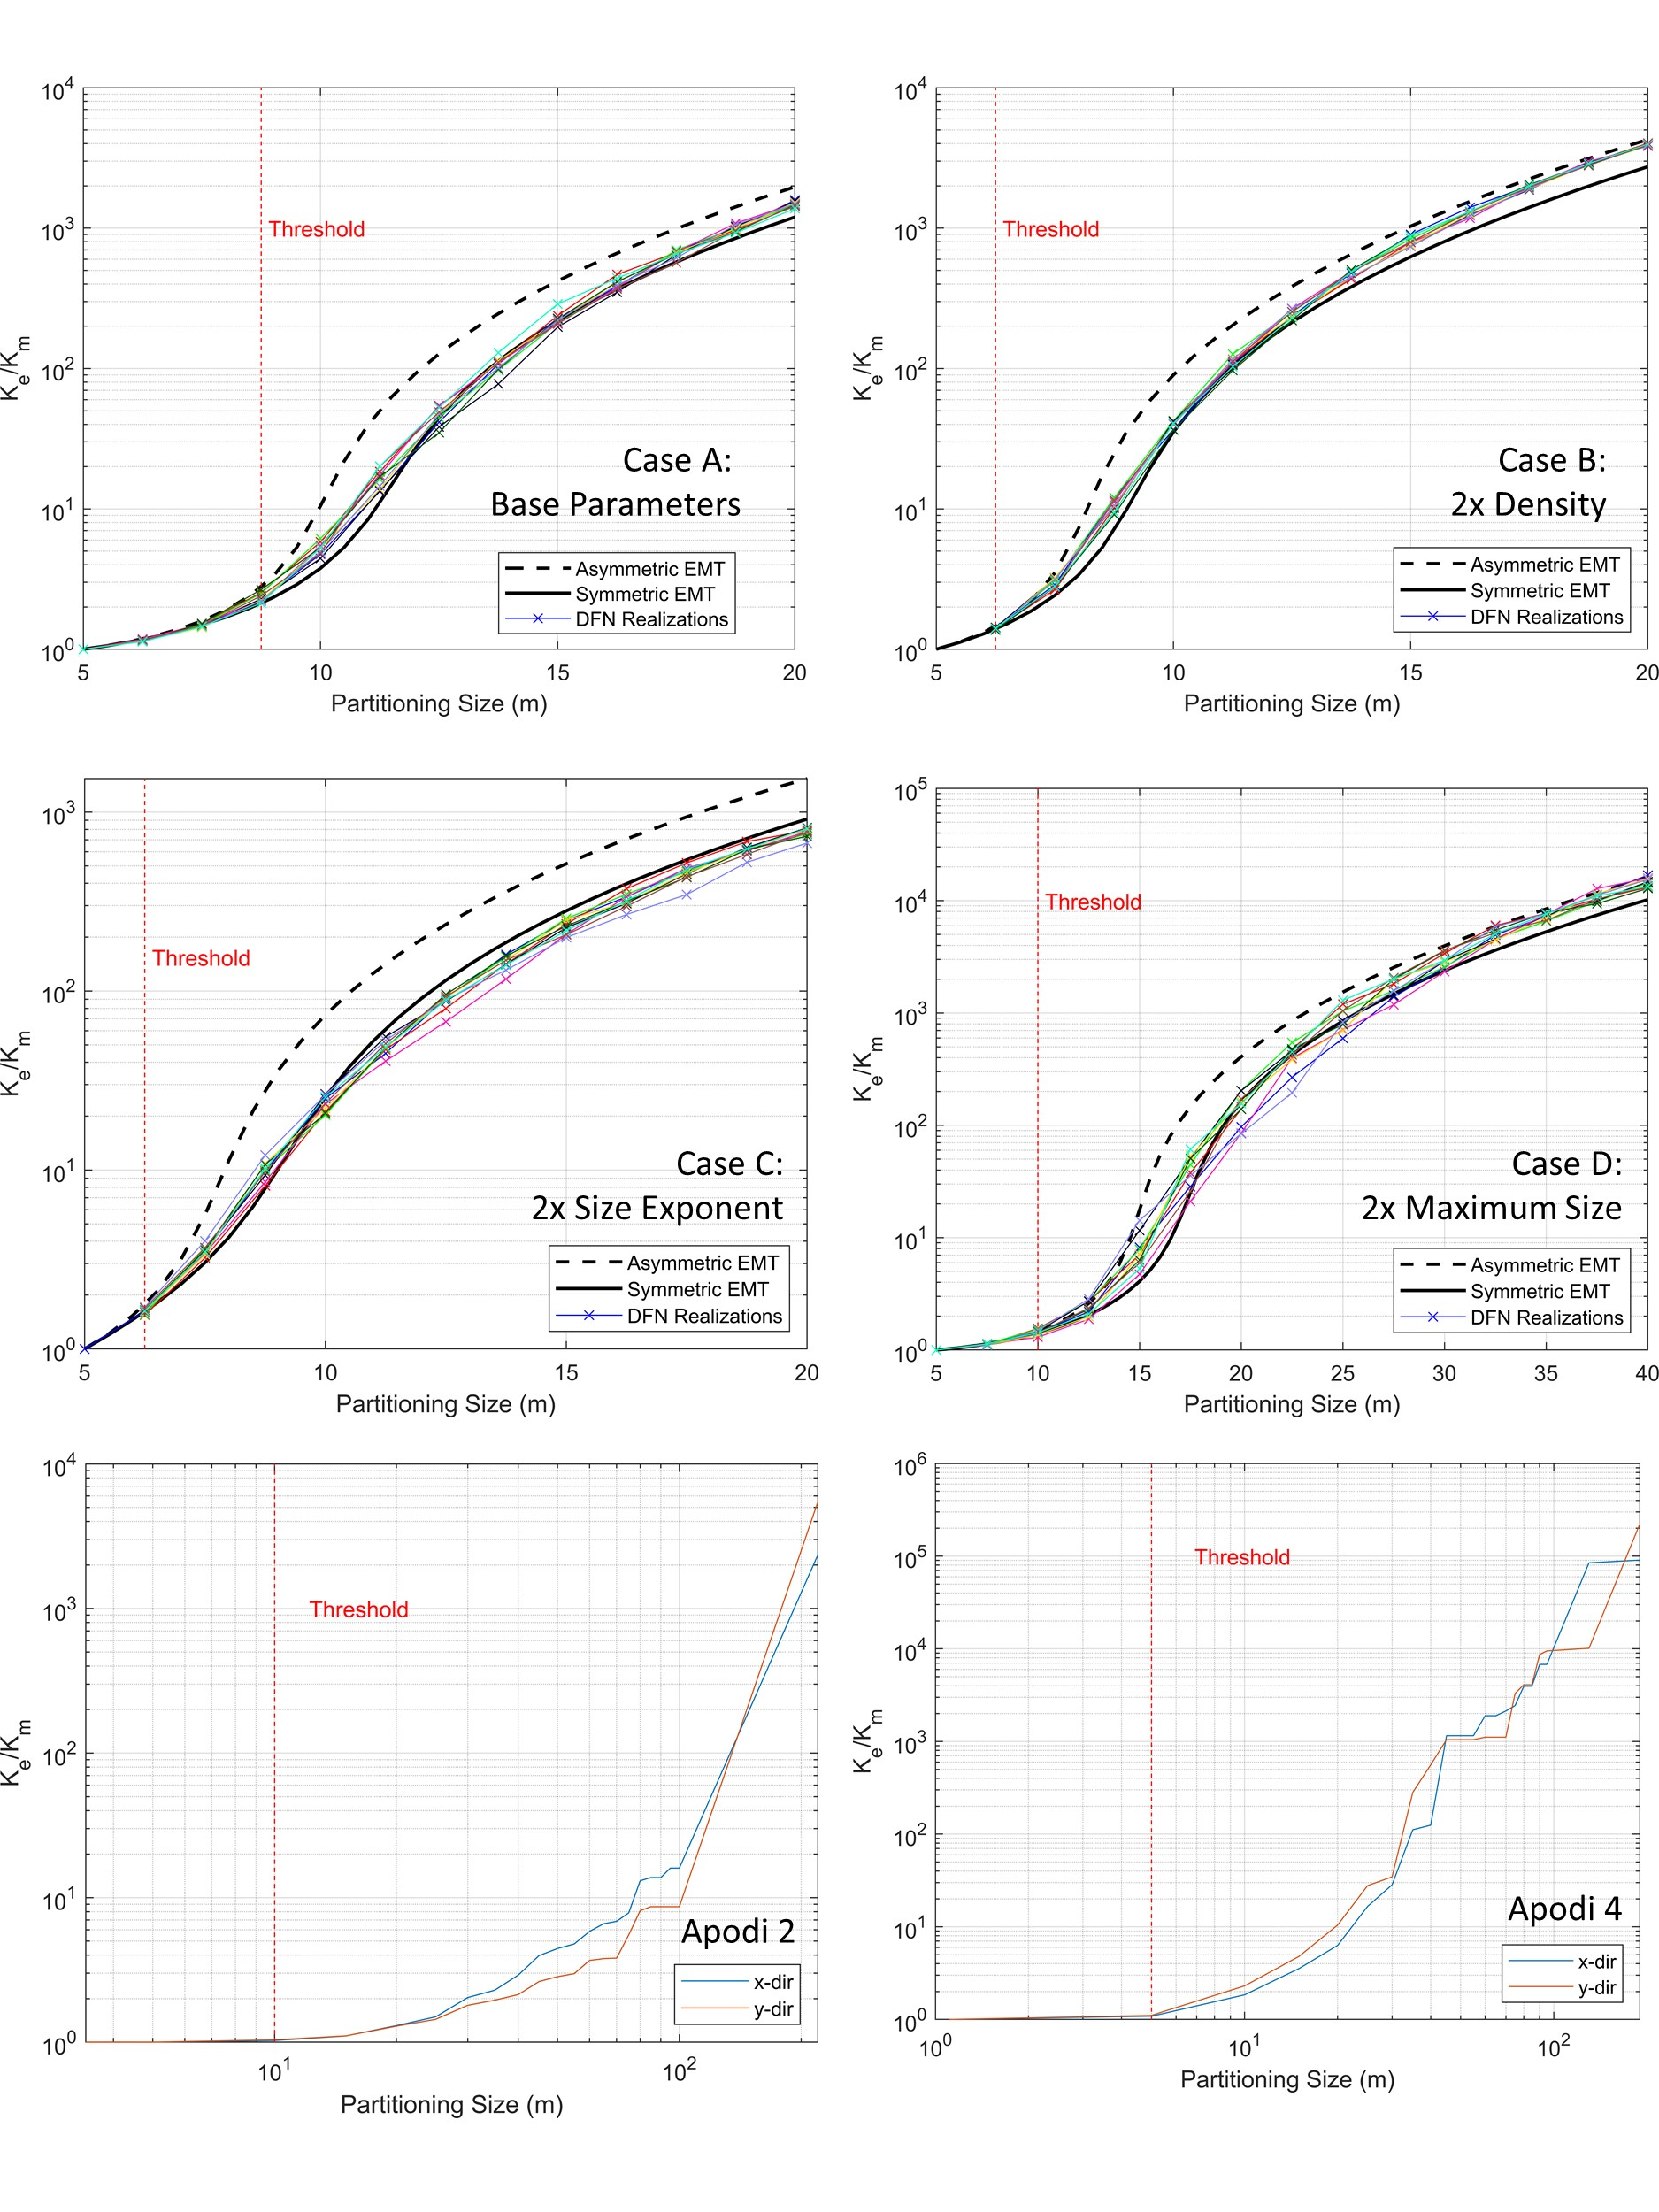
\includegraphics[width=\textwidth]{FSU_main_V.jpg}

 \caption{Fracture Subset Upscaling. Cases A to D correspond to generated 3D DFNs. Apodi 2 and 4 are based on outcrop fracture data. Threshold partitioning sizes, $s_p^*$, calculated using both numerical and analytical approaches are shown.}
 \label{fig:FSU}
\end{figure}

\subsection{Single Phase Flow in Hybrid Models}
In Figure \ref{fig:DD}, we show the results for six drawdown studies based on our datasets. We further performed eleven drawdown studies that are shown in Figures S2 and S3. In all studies, we show full model solutions based on the original non-upscaled data; these serve as reference solutions. All other solutions are generated from hybrid models corresponding to different $s_p$ values. 

A fixed pressure boundary ($50$ bars) is used to initiate a drawdown for the 3D DFNs. Hence the plots show outlet flowrate against time. Due to the high fracture-to-rock permeability ratio, the pressure drop preferentially diffuses through the fracture network. When pressure in the fractures depletes significantly, fluid in the rock matrix begins to recharge the fracture network. This results in a stationary flow regime (Cases A to D in Figure \ref{fig:DD}, and Figure S2). Finally, when pressure in the entire model depletes, flowrate at the outlet goes to zero.

For Apodi 2 (Figure \ref{fig:DD}), a well is positioned in the rock matrix and drawn down at a fixed rate ($0.1$m\textsuperscript{3}/day). The pressure derivative response initially shows a straight line due to the wellbore storage effect as pressure is depleted in the well. We then observe an infinite acting regime when the perturbation at the well only diffuses through the matrix; this corresponds to the flat plateau in the derivative plot. Once the effect of the well drawdown reaches the nearest fracture, fluid depletion from the fracture network dominates due to the high fracture conductivities. This results in a dip on the pressure derivative \citep{Bourdet1989, Egya2018}. For Apodi 4, the behaviour is similar (Figure S3).

In another test, we positioned a well to intersect the largest fracture in Apodi 4 and drew down at a fixed rate ($1$m\textsuperscript{3}/day) (Figure \ref{fig:DD}). In this setup, there is similarly an initial wellbore storage effect which manifests itself in a straight line. The pressure drop at the well then diffuses through the fracture network. In this regime, the rock matrix is effectively impermeable. Once the pressure diffusion reaches the boundaries, fluid pressure in the fractures begin to drop significantly. The fluid contained in the rock matrix then begins to recharge the fracture network. This results in a dip on the pressure derivative as well \citep{Gringarten1987}. For Apodi 2, the behaviour is similar (Figure S3).

In all drawdown studies, the differences between hybrid and full model results are minimal for small $s_p$ values. However, it is observed that as $s_p$ increases, the corresponding hybrid model produces results that deviate more from the reference solution (Figure \ref{fig:DD}). The flowrate or pressure derivative mismatch (Figure \ref{fig:HP}) generally shows the same trend. As the mismatch is measured at a fixed point in time, the mismatch seemingly decreases for some cases at large $s_p$ values. However, Figure \ref{fig:DD} shows that the overall drawdown response of the hybrid models continuously deviate away from the reference solutions. 

In terms of model simplification, the number of fractures, fracture grid cells and NNCs all decrease as $s_p$ is increased (Figure \ref{fig:HP}), which suggests a trade-off relationship between model simplicity and accuracy. Large $s_p$ values result in simpler models with less explicit fractures that produce less accurate results. In practice, we seek an intermediate $s_p$ which allows us to balance both needs. It is noteworthy that for small $s_p$ values, as $s_p$ increases, the percentage reduction in fractures, fracture cells and NNCs exceeds the increase in flowrate or pressure derivative mismatch. This favourable trade-off ascertains that hybrid models do have the capability to simplify simulations while preserving accuracy. In section \ref{discussion}, we will discuss how to choose an appropriate $s_p$ value without having to perform any flow simulations.

\begin{figure}[h]
	\centering
	
	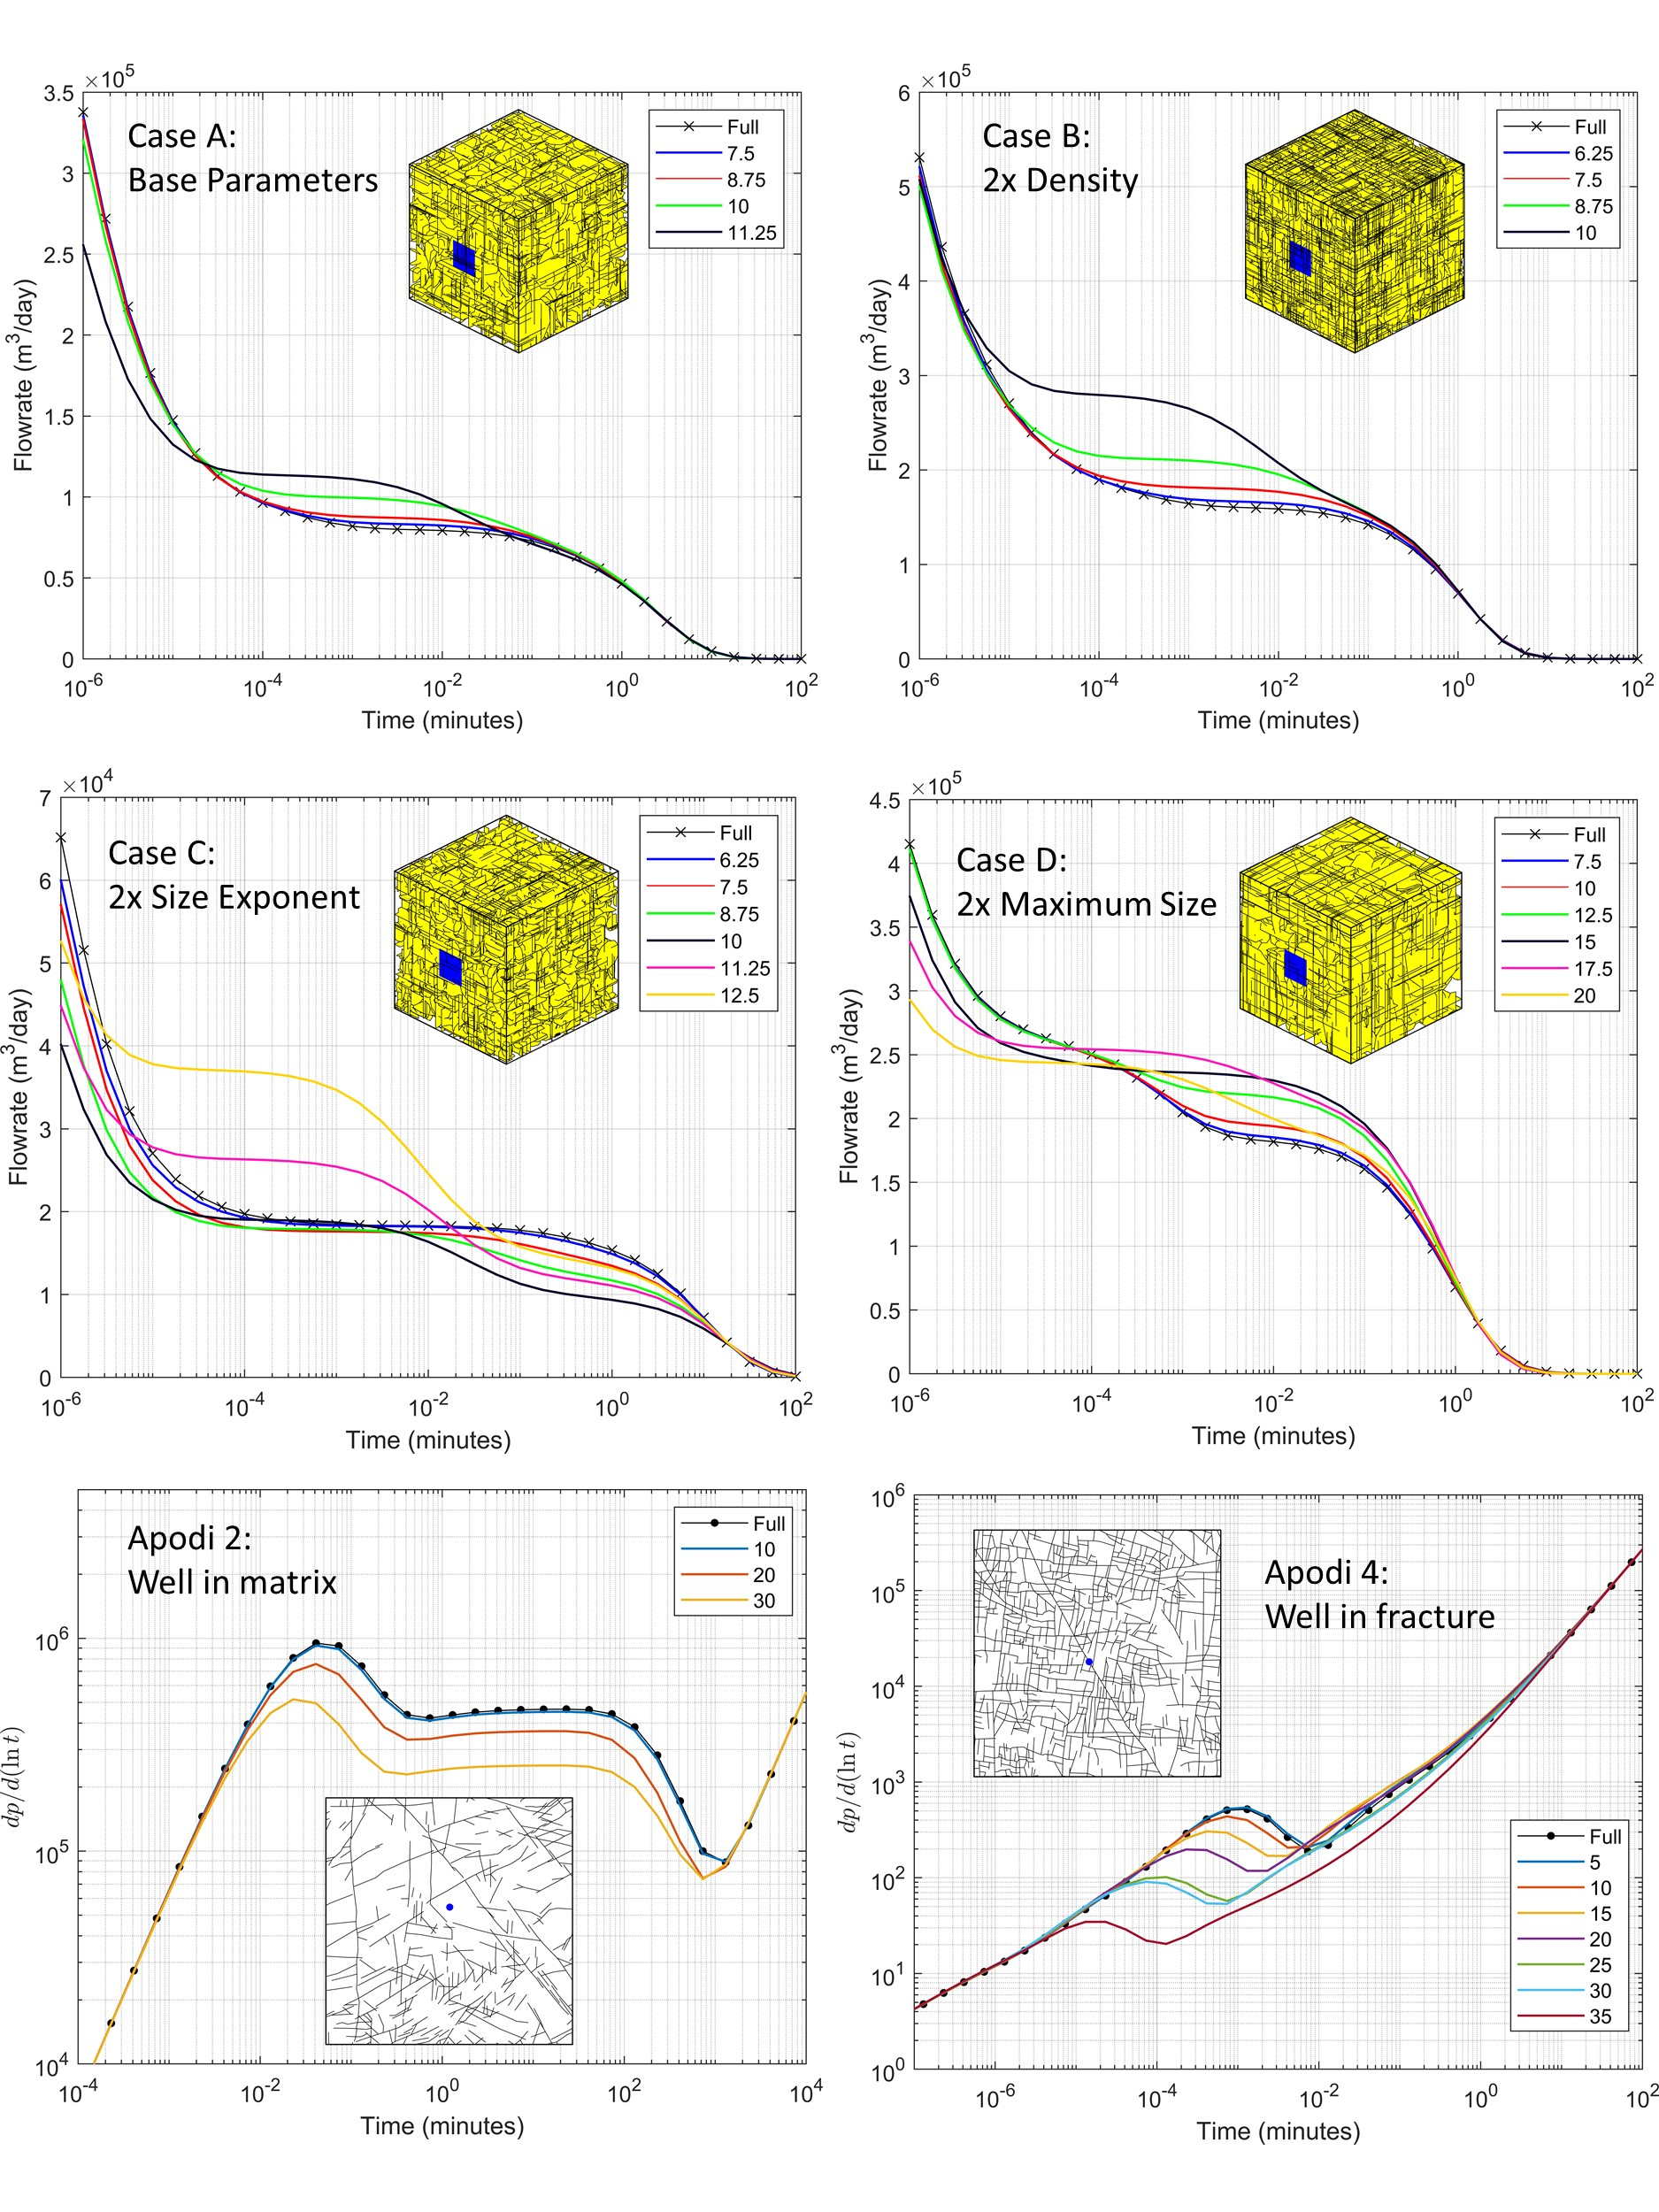
\includegraphics[width=\textwidth]{DD_main_V.jpg}
	
	\caption{Drawdown curves for fully resolved models, and hybrid models corresponding to different partitioning sizes. Cases A to D: Fixed pressure is applied on blue faces. Domain size is 100m x 100m x 100m in all cases. Apodi 2 and 4: Fixed flowrate is applied at locations marked with blue circle. Domain size is 220m x 220m x 1m and 100m x 100m x 1m for Apodi 2 and 4 respectively.}
	\label{fig:DD}
\end{figure}

\begin{figure}[h]
	\centering
	
	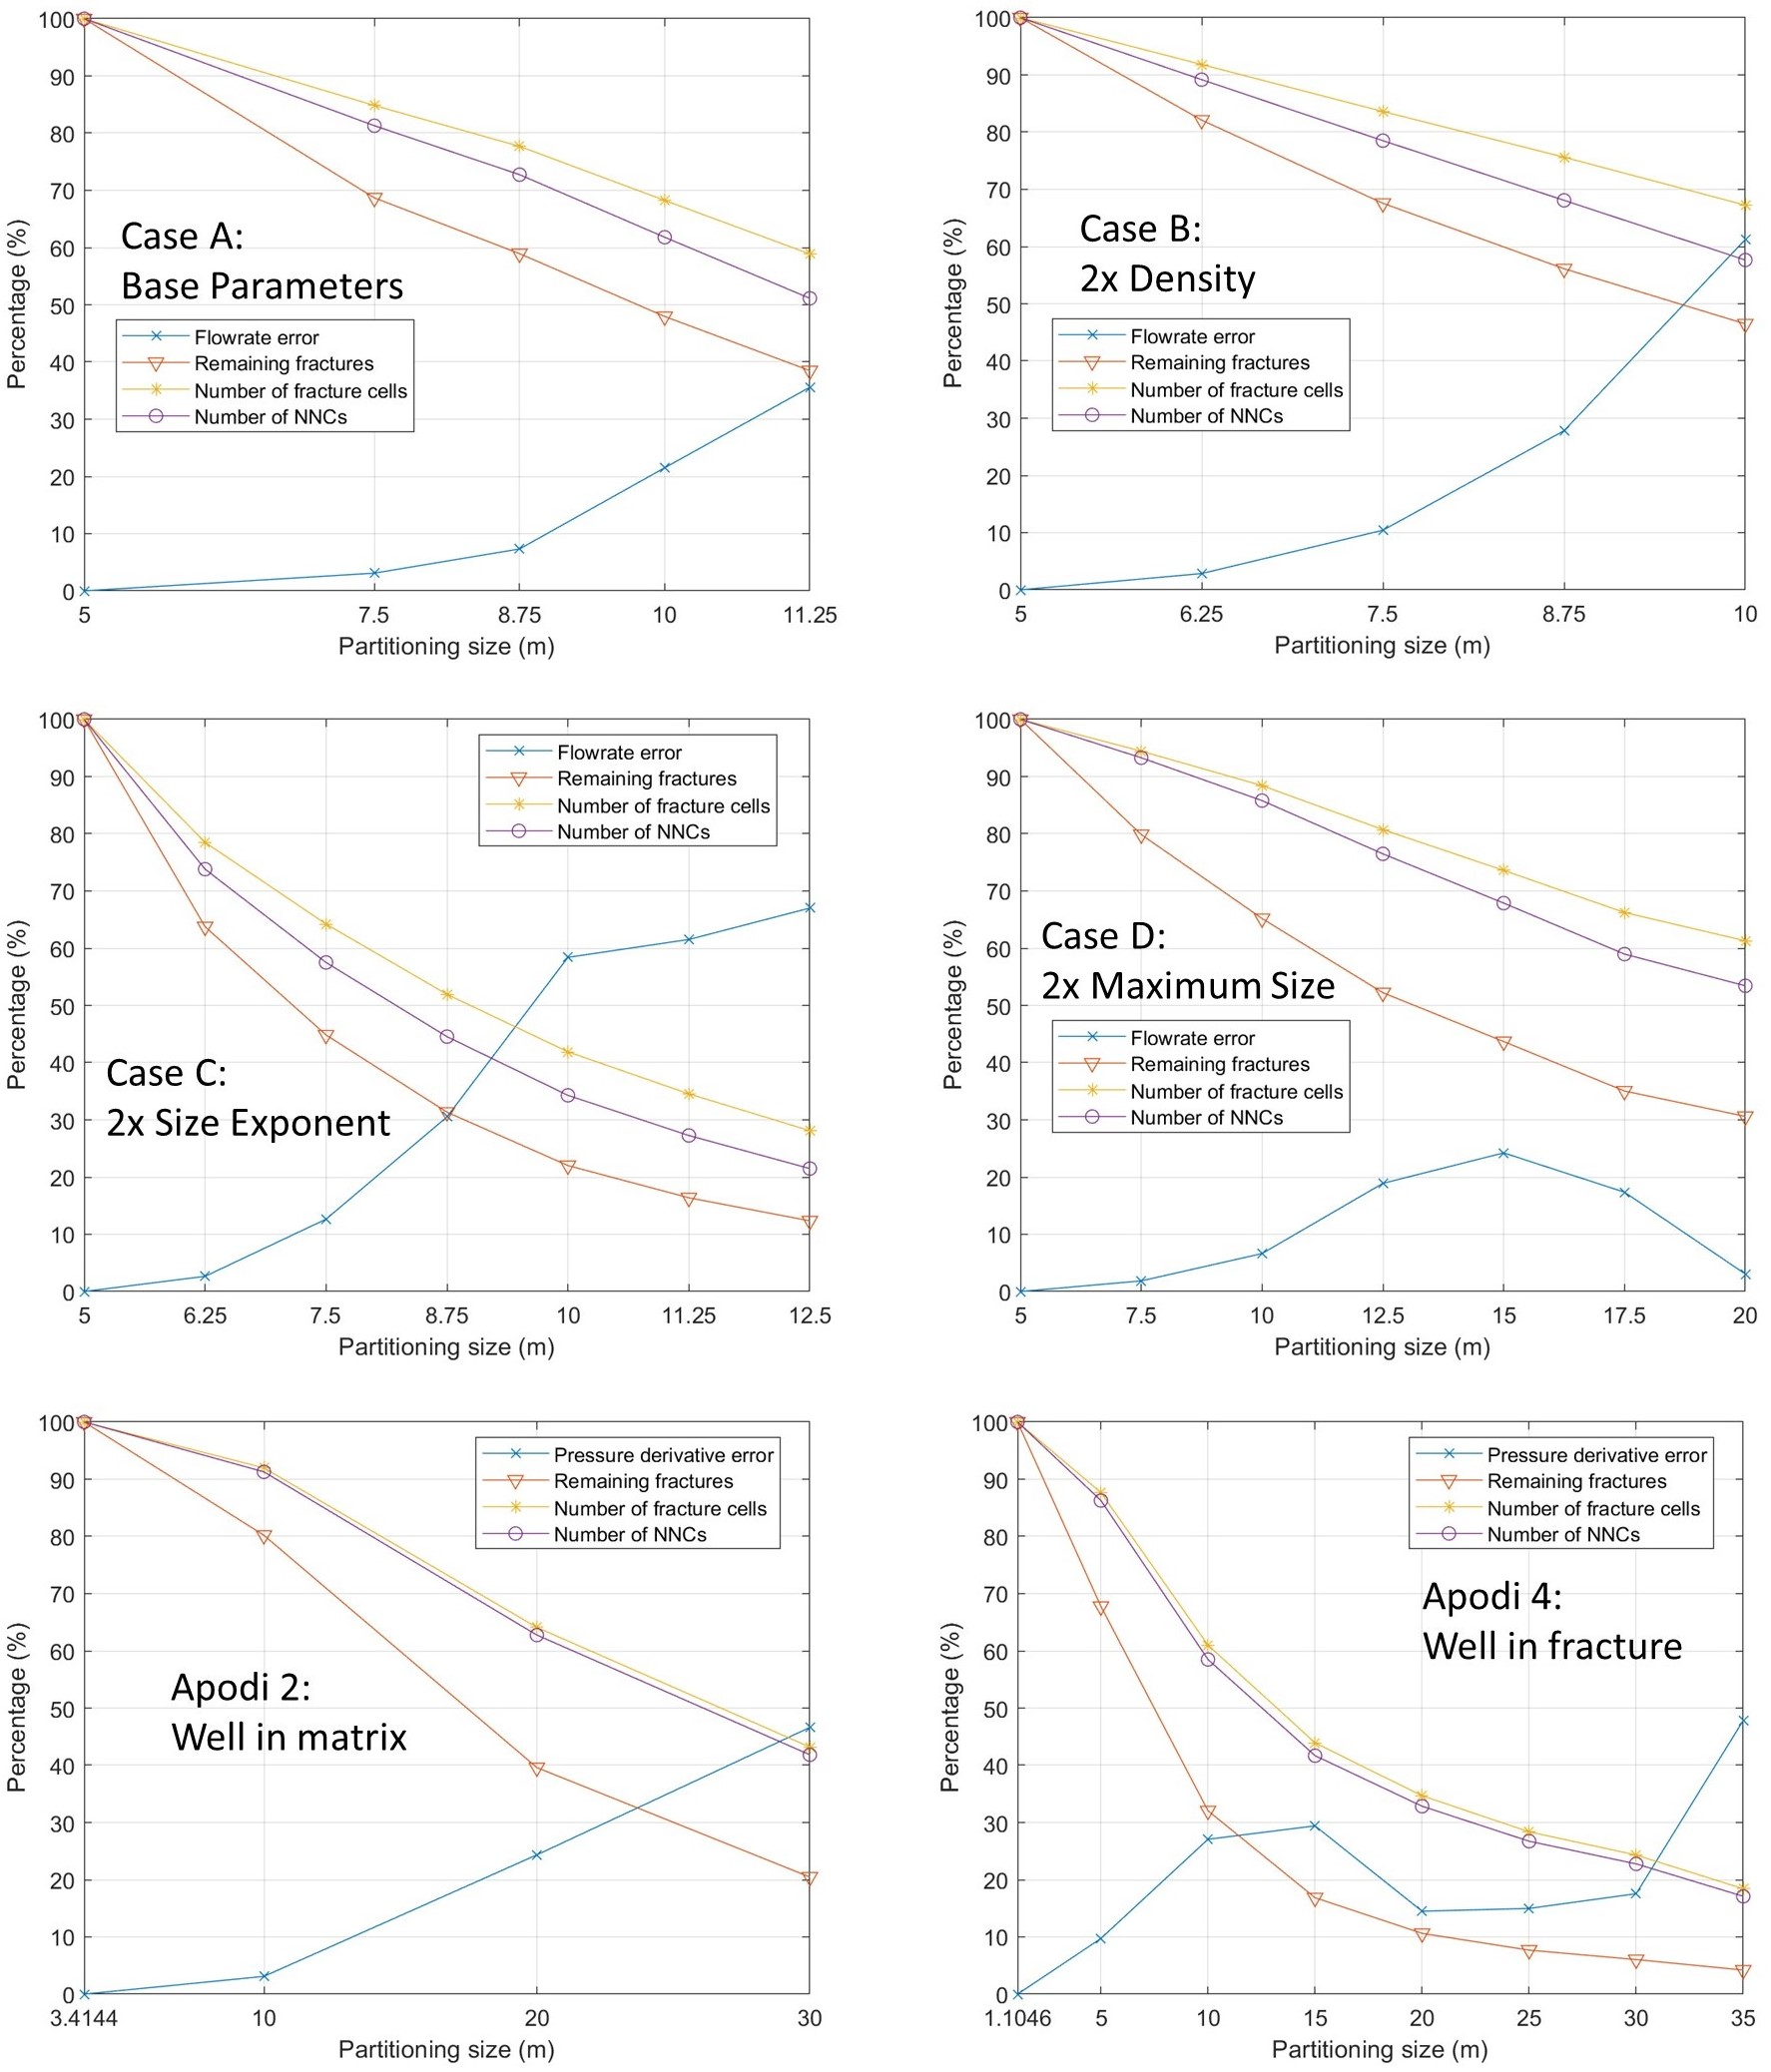
\includegraphics[width=\textwidth]{Hybrid_Perf.jpg}
	
	\caption{Errors and simplifications due to hybrid modelling. Errors are calculated at $0.001$ minutes for Case A, $0.001$ minutes for Case B, $0.1$ minutes for Case C, $0.01$ minutes for Case D, $73.2$ minutes for Apodi 2, and $0.0412$ minutes for Apodi 4.}
	\label{fig:HP}
\end{figure}

\subsection{Accuracy of Effective Medium Theory}
The FSU curves generated for the 3D DFNs using the Effective Medium Theory are also shown in Figures \ref{fig:FSU} and S1. In general, there is a good match between the results obtained from both numerical and analytical approaches. Furthermore, the results show that FSU results from the Effective Medium Theory are representative of different stochastic realizations of the same fracture network parameter set. We observe that the symmetric self-consistent method performs best in terms of overall $K_e$ calculations, especially at low partitioning sizes; this is in line with \citet{Saevik2013}'s observations since we are upscaling subsets of the full fracture network. We also note that the asymmetric self-consistent method tends to over-estimates $K_e$. At high densities (Case B), however, the asymmetric self-consistent method is more accurate at high $s_p$ values.

The ability of the Effective Medium Theory to capture the percolation behaviour in the FSU curves is noteworthy since its mathematical formulation does not account for fracture network topology. This has similarly been observed by \citet{Saevik2013} and no explanation has been provided yet.

The main limitation that prevents the Effective Medium Theory from being used for the Apodi 2 and 4 datasets is that it does not take into consideration the abutment relationships between fracture sets. However, in our studies, the Effective Medium Theory is significantly more efficient than numerical flow based upscaling and reduces the FSU processing time from hours to seconds.

\section{Discussion}
\label{discussion}

\subsection{Effect of Partitioning Size on Accuracy of Simulation Results}
Using the drawdown studies, we established that there is a trade-off between model simplicity and accuracy. As such, we seek an intermediate $s_p$ value that strikes a balance between the two. How can we know \textit{a priori} whether or not a selected $s_p$ is applicable for single porosity hybrid modelling? Might it results in an oversimplification? Or will it adequately preserve the fidelity of the model? 

We previously hypothesized that the threshold partitioning size $s_p^*$ determined from FSU can be used to determine if a single porosity hybrid model is applicable for a given partitioning size. The values for $s_p^*$ are shown in Figures \ref{fig:FSU} and S1. Based on the drawdown results in Figures \ref{fig:DD}, \ref{fig:HP}, S2 and S3, it can be seen that hybrid models corresponding to $s_p \leq s_p^*$ produce results that are very similar to the reference full model solution. On the other hand, hybrid model solutions corresponding to $s_p > s_p^*$ begin to deviate significantly from the reference solutions. These results show that $s_p^*$ determined from FSU are effective in evaluating the suitability of a partitioning threshold for single porosity hybrid modelling. The efficacy of $s_p^*$ is due to its association with the percolation behaviour observed in the permeability-size relationships. In order for a single porosity representation to be valid, we have to ensure that there is no separation of scale between fluid flow in the matrix and the upscaled fracture network \citep{Matthai2004a}. For low $s_p$ values, the small fractures are disperse and poorly connected. Pressure perturbations diffuse through the rock matrix and small fractures at almost equal rates. However, for high $s_p$ values, the small fractures are abundant and become well connected. In this case, pressure perturbations will preferentially diffuse through the small fractures before affecting the fluid in the rock. $s_p^*$ is the threshold where the small fractures begin to be connected. Therefore, $s_p$ must be smaller than $s_p^*$ to obtain an accurate single porosity hybrid model.

From a pragmatic viewpoint, a threshold partitioning size $s_p^*$ implies a limit to how much we can simplify our simulation model. This is because as $s_p$ increases beyond $s_p^*$, we begin to reduce computational load at the expense of model accuracy. In practice, determining $s_p^*$ allows us to assess our modelling approach. If the simulation grid size used in a model is smaller than $s_p^*$, we can be sure that upscaling fractures smaller than the grid cell will not negatively impact model accuracy.

\subsection{\textit{A priori} Identification of Partitioning Threshold}
In Figures \ref{fig:DD}, \ref{fig:HP}, S2 and S3, we showed that not all partitioning sizes are suitable for single porosity hybrid modelling. As a simulation practitioner, one possible way to take to determine the range of appropriate values for $s_p$ is to use a trial-and-error approach, where hybrid models with different partitioning sizes are compared to fully resolved models. 

In practice, this is a time consuming process and will not be useful. Based on the work presented in this paper, we propose to use FSU to determine the range of $s_p$ suitable for single porosity hybrid modelling. We do this by exploiting the percolation behaviour observed in the FSU curves. In general, FSU can be performed numerically for all types of fracture networks. Once the FSU curves are calculated, $s_p^*$ can be identified. Any $s_p$ value less than $s_p^*$ can then be used to construct single porosity hybrid models. As shown in Figures \ref{fig:DD}, \ref{fig:HP}, S2 and S3, such single porosity hybrid models will be able to match fully resolved models in terms of output accuracy.

To further expedite this decision making process, we also advocate using the Effective Medium Theory for FSU whenever possible. Since the Effective Medium Theory is a semi-analytical upscaling tool, it produces results in a matter of seconds. By comparison, the numerical approach takes hours to complete due to preprocessing requirements such as grid construction and the establishment of matrix-fracture and fracture-fracture connections. As was shown in Figures \ref{fig:FSU} and S1, for uncorrelated fracture sets, with fractures uniformly distributed in space, performing FSU with the Effective Medium Theory yields results that match numerical flow based upscaling. In reality, fracture networks may be less conductive than predicted by the theory. This is because fracture sets are usually correlated with each other through abutment relationships. This correlation results in less intersections per fracture than expected. Research is ongoing to incorporate such relationships in analytical upscaling tools \citep{Hardebol2015, Makel2007, Saevik2017}. 

% Adjust conclusions to changes made so far.

\section{Conclusion}
Fluid flow modelling in naturally fractured reservoirs is a challenging process due to the multiscale nature of fractures. One of the major difficulties is the accurate representation of multiscale fractures in simulation models. Single porosity hybrid models that represent small fractures implicitly and large fractures explicitly are useful in this regard. Splitting a fracture set into small and large sets requires the choice of a partitioning size.

We conducted numerical studies using synthetic 3D and outcrop based 2D datasets. The drawdown simulations performed on full non-upscaled, and hybrid models confirm that hybrid models created with partitioning sizes do reduce simulation complexity while maintaining accuracy of outputs. However, partitioning sizes must not be unreasonably large. In fact, for each dataset, we identified a threshold partitioning size beyond which single porosity hybrid models become significantly inaccurate.

For every dataset, we can identify the threshold partitioning size by solving the Laplace equation either numerically or analytically. By upscaling small fractures with the rock matrix, we obtain effective permeabilities that depend on partitioning size. This permeability-size relationship is also referred to as a Fracture Subset Upscaling curve. The threshold partitioning size coincides with the point on the curve where effective permeability of small fractures begins to increase significantly. 

Finally, we also note that Fracture Subset Upscaling can be performed \textit{a priori} and efficiently using the Effective Medium Theory, which is a semi-analytical upscaling tool. This technique reduces the time needed to generate the permeability-size relationship from hours to seconds. However, the Effective Medium Theory currently does not take into consideration geological features such as abutment relationships and non-uniform spatial distributions of fractures. Where necessary, numerical flow based upscaling can also be used for Fracture Subset Upscaling. In terms of fracture network properties, a numerical approach is less restrictive, but is significantly more resource intensive.
%Text here ===>>>

%%

%  Numbered lines in equations:
%  To add line numbers to lines in equations,
%  \begin{linenomath*}
%  \begin{equation}
%  \end{equation}
%  \end{linenomath*}



%% Enter Figures and Tables near as possible to where they are first mentioned:
%
% DO NOT USE \psfrag or \subfigure commands.
%
% Figure captions go below the figure.
% Table titles go above tables;  other caption information
%  should be placed in last line of the table, using
% \multicolumn2l{$^a$ This is a table note.}
%
%----------------
% EXAMPLE FIGURE
%
% \begin{figure}[h]
% \centering
% when using pdflatex, use pdf file:
% \includegraphics[natwidth=800px,natheight=600px]{figsamp.pdf}
%
% when using dvips, use .eps file:
% \includegraphics[natwidth=800px,natheight=600px]{figsamp.eps}
%
% \caption{Short caption}
% \label{figone}
%  \end{figure}
%
% We recommend that you provide the native width and height (natwidth, natheight) of your figures.
% Specifying native dimensions ensures that your figures are properly scaled
%
%
% ---------------
% EXAMPLE TABLE
%
% \begin{table}
% \caption{Time of the Transition Between Phase 1 and Phase 2$^{a}$}
% \centering
% \begin{tabular}{l c}
% \hline
%  Run  & Time (min)  \\
% \hline
%   $l1$  & 260   \\
%   $l2$  & 300   \\
%   $l3$  & 340   \\
%   $h1$  & 270   \\
%   $h2$  & 250   \\
%   $h3$  & 380   \\
%   $r1$  & 370   \\
%   $r2$  & 390   \\
% \hline
% \multicolumn{2}{l}{$^{a}$Footnote text here.}
% \end{tabular}
% \end{table}

%% SIDEWAYS FIGURE and TABLE
% AGU prefers the use of {sidewaystable} over {landscapetable} as it causes fewer problems.
%
% \begin{sidewaysfigure}
% \includegraphics[width=20pc]{figsamp}
% \caption{caption here}
% \label{newfig}
% \end{sidewaysfigure}
%
%  \begin{sidewaystable}
%  \caption{Caption here}
% \label{tab:signif_gap_clos}
%  \begin{tabular}{ccc}
% one&two&three\\
% four&five&six
%  \end{tabular}
%  \end{sidewaystable}

%% If using numbered lines, please surround equations with \begin{linenomath*}...\end{linenomath*}
%\begin{linenomath*}
%\begin{equation}
%y|{f} \sim g(m, \sigma),
%\end{equation}
%\end{linenomath*}

%%% End of body of article

%%%%%%%%%%%%%%%%%%%%%%%%%%%%%%%%
%% Optional Appendix goes here
%
% The \appendix command resets counters and redefines section heads
%
% After typing \appendix
%
%\section{Here Is Appendix Title}
% will show
% A: Here Is Appendix Title
%
%\appendix
%\section{Here is a sample appendix}

%%%%%%%%%%%%%%%%%%%%%%%%%%%%%%%%%%%%%%%%%%%%%%%%%%%%%%%%%%%%%%%%
%
% Optional Glossary, Notation or Acronym section goes here:
%
%%%%%%%%%%%%%%
% Glossary is only allowed in Reviews of Geophysics
%  \begin{glossary}
%  \term{Term}
%   Term Definition here
%  \term{Term}
%   Term Definition here
%  \term{Term}
%   Term Definition here
%  \end{glossary}

%
%%%%%%%%%%%%%%
% Acronyms
%   \begin{acronyms}
%   \acro{Acronym}
%   Definition here
%   \acro{EMOS}
%   Ensemble model output statistics
%   \acro{ECMWF}
%   Centre for Medium-Range Weather Forecasts
%   \end{acronyms}

%
%%%%%%%%%%%%%%
% Notation
%   \begin{notation}
%   \notation{$a+b$} Notation Definition here
%   \notation{$e=mc^2$}
%   Equation in German-born physicist Albert Einstein's theory of special
%  relativity that showed that the increased relativistic mass ($m$) of a
%  body comes from the energy of motion of the body—that is, its kinetic
%  energy ($E$)—divided by the speed of light squared ($c^2$).
%   \end{notation}




%%%%%%%%%%%%%%%%%%%%%%%%%%%%%%%%%%%%%%%%%%%%%%%%%%%%%%%%%%%%%%%%
%
%  ACKNOWLEDGMENTS
%
% The acknowledgments must list:
%
% >>>>	A statement that indicates to the reader where the data
% 	supporting the conclusions can be obtained (for example, in the
% 	references, tables, supporting information, and other databases).
%
% 	All funding sources related to this work from all authors
%
% 	Any real or perceived financial conflicts of interests for any
%	author
%
% 	Other affiliations for any author that may be perceived as
% 	having a conflict of interest with respect to the results of this
% 	paper.
%
%
% It is also the appropriate place to thank colleagues and other contributors.
% AGU does not normally allow dedications.


\acknowledgments
The authors are grateful to Total, S.A. for funding Daniel Wong's PhD research. We also thank Energi Simulation for funding Sebastian Geiger's Chair in Carbonate Reservoir Simulation. Finally, we thank TU Delft for making their datasets available through \citet{Bisdom2017}.


%% ------------------------------------------------------------------------ %%
%% References and Citations

%%%%%%%%%%%%%%%%%%%%%%%%%%%%%%%%%%%%%%%%%%%%%%%
% BibTeX is preferred:
%
% \bibliography{<name of your .bib file>}
%
% don't specify bibliographystyle
%%%%%%%%%%%%%%%%%%%%%%%%%%%%%%%%%%%%%%%%%%%%%%%

\bibliography{library}

% Please use ONLY \citet and \citep for reference citations.
% DO NOT use other cite commands (e.g., \cite, \citeyear, \nocite, \citealp, etc.).
%% Example \citet and \citep:
%  ...as shown by \citet{Boug10}, \citet{Buiz07}, \citet{Fra10},
%  \citet{Ghel00}, and \citet{Leit74}.

%  ...as shown by \citep{Boug10}, \citep{Buiz07}, \citep{Fra10},
%  \citep{Ghel00, Leit74}.

%  ...has been shown \citep [e.g.,][]{Boug10,Buiz07,Fra10}.


\end{document}



More Information and Advice:

%% ------------------------------------------------------------------------ %%
%
%  SECTION HEADS
%
%% ------------------------------------------------------------------------ %%

% Capitalize the first letter of each word (except for
% prepositions, conjunctions, and articles that are
% three or fewer letters).

% AGU follows standard outline style; therefore, there cannot be a section 1 without
% a section 2, or a section 2.3.1 without a section 2.3.2.
% Please make sure your section numbers are balanced.
% ---------------
% Level 1 head
%
% Use the \section{} command to identify level 1 heads;
% type the appropriate head wording between the curly
% brackets, as shown below.
%
%An example:
%\section{Level 1 Head: Introduction}
%
% ---------------
% Level 2 head
%
% Use the \subsection{} command to identify level 2 heads.
%An example:
%\subsection{Level 2 Head}
%
% ---------------
% Level 3 head
%
% Use the \subsubsection{} command to identify level 3 heads
%An example:
%\subsubsection{Level 3 Head}
%
%---------------
% Level 4 head
%
% Use the \subsubsubsection{} command to identify level 3 heads
% An example:
%\subsubsubsection{Level 4 Head} An example.
%
%% ------------------------------------------------------------------------ %%
%
%  IN-TEXT LISTS
%
%% ------------------------------------------------------------------------ %%
%
% Do not use bulleted lists; enumerated lists are okay.
% \begin{enumerate}
% \item
% \item
% \item
% \end{enumerate}
%
%% ------------------------------------------------------------------------ %%
%
%  EQUATIONS
%
%% ------------------------------------------------------------------------ %%

% Single-line equations are centered.
% Equation arrays will appear left-aligned.

Math coded inside display math mode \[ ...\]
 will not be numbered, e.g.,:
 \[ x^2=y^2 + z^2\]

 Math coded inside \begin{equation} and \end{equation} will
 be automatically numbered, e.g.,:
 \begin{equation}
 x^2=y^2 + z^2
 \end{equation}


% To create multiline equations, use the
% \begin{eqnarray} and \end{eqnarray} environment
% as demonstrated below.
\begin{eqnarray}
  x_{1} & = & (x - x_{0}) \cos \Theta \nonumber \\
        && + (y - y_{0}) \sin \Theta  \nonumber \\
  y_{1} & = & -(x - x_{0}) \sin \Theta \nonumber \\
        && + (y - y_{0}) \cos \Theta.
\end{eqnarray}

%If you don't want an equation number, use the star form:
%\begin{eqnarray*}...\end{eqnarray*}

% Break each line at a sign of operation
% (+, -, etc.) if possible, with the sign of operation
% on the new line.

% Indent second and subsequent lines to align with
% the first character following the equal sign on the
% first line.

% Use an \hspace{} command to insert horizontal space
% into your equation if necessary. Place an appropriate
% unit of measure between the curly braces, e.g.
% \hspace{1in}; you may have to experiment to achieve
% the correct amount of space.


%% ------------------------------------------------------------------------ %%
%
%  EQUATION NUMBERING: COUNTER
%
%% ------------------------------------------------------------------------ %%

% You may change equation numbering by resetting
% the equation counter or by explicitly numbering
% an equation.

% To explicitly number an equation, type \eqnum{}
% (with the desired number between the brackets)
% after the \begin{equation} or \begin{eqnarray}
% command.  The \eqnum{} command will affect only
% the equation it appears with; LaTeX will number
% any equations appearing later in the manuscript
% according to the equation counter.
%

% If you have a multiline equation that needs only
% one equation number, use a \nonumber command in
% front of the double backslashes (\\) as shown in
% the multiline equation above.

% If you are using line numbers, remember to surround
% equations with \begin{linenomath*}...\end{linenomath*}

%  To add line numbers to lines in equations:
%  \begin{linenomath*}
%  \begin{equation}
%  \end{equation}
%  \end{linenomath*}



